\begin{figure}[tb]
 \centering % avoid the use of \begin{center}...\end{center} and use \centering instead (more compact)
 \includegraphics[width=\columnwidth]{pictures/01-initial-correlation.png}
 \caption{Linear Regression for 6 sample log files, with lines of best fit and correlation coefficients. Top left plot (1) is real fire data. Plots 3 and 5 are pure acquisitions, with no fire or interference.}
 \label{fig:sample}
\end{figure}


\begin{figure}[tb]
 \centering % avoid the use of \begin{center}...\end{center} and use \centering instead (more compact)
 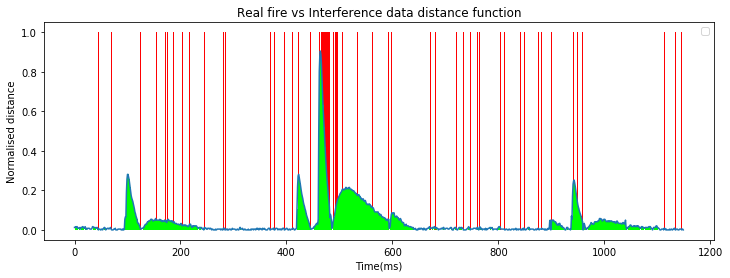
\includegraphics[width=\columnwidth]{pictures/02-area-to-filter.png}
 \caption{Plot showing distance function (blue), antiphase between channels (red) and area to be smoothed (green).}
 \label{fig:sample}
\end{figure}


\begin{figure}[tb]
 \centering % avoid the use of \begin{center}...\end{center} and use \centering instead (more compact)
 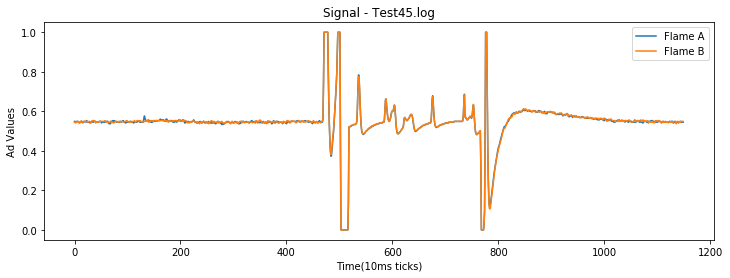
\includegraphics[width=\columnwidth]{pictures/05-signal.png}
 \caption{Signal data, generated by waving a barbecue lighter in front of UUT}
 \label{fig:sample}
\end{figure}

\begin{figure}[tb]
 \centering % avoid the use of \begin{center}...\end{center} and use \centering instead (more compact)
 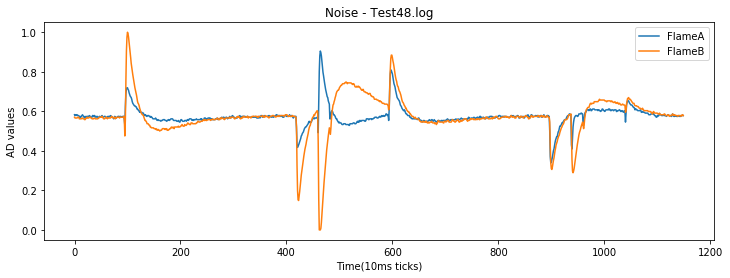
\includegraphics[width=\columnwidth]{pictures/04-noise.png}
 \caption{Noise data, generated by RF interference}
 \label{fig:sample}
\end{figure}

\begin{figure}[tb]
 \centering % avoid the use of \begin{center}...\end{center} and use \centering instead (more compact)
 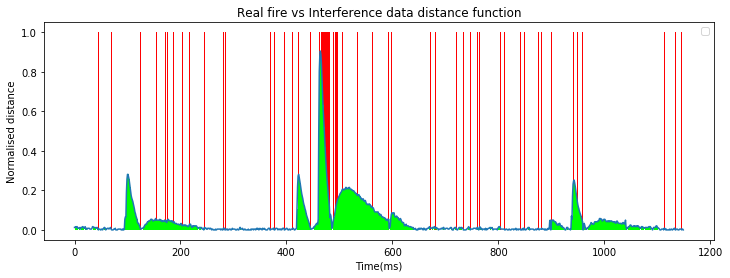
\includegraphics[width=\columnwidth]{pictures/02-area-to-filter.png}
 \caption{Plot showing distance function (blue), antiphase between channels (red) and area to be smoothed (green).}
 \label{fig:sample}
\end{figure}